\documentclass{article}
\usepackage{graphicx}
\usepackage{listings}
\usepackage{color}
\usepackage[utf8]{inputenc}

\title{Sperimentazione sull'influenza del parametro $\gamma$ sull'ordinamento del PageRank\\
	Corso di LSMC, a.a. 2017-2018}
\author{Davide Gori\\
	550282}


\definecolor{backcolour}{rgb}{0.95,0.95,0.92}
\definecolor{gray}{rgb}{0.5,0.5,0.5}
\lstset{basicstyle=\ttfamily\small,
	columns=fullflexible,
	numbers=left,
	numberstyle=\tiny\ttfamily\color{gray},
	backgroundcolor=\color{backcolour},
	tabsize=4,
	language=Octave
}


\begin{document}
	\maketitle
	
	\section{Obiettivi e descrizione della sperimentazione}
	Vogliamo valutare come e quanto il parametro $\gamma$ influenza l'ordinamento PageRank. In particolare confronteremo il caso $\gamma=0.85$ (valore consigliato da Google) e il caso $\gamma=0.99$ (in cui il vettore di personalizzazione ha una bassa incidenza).\\

	\section{Sperimentazione}
	Generiamo una matrice di adiacenza con $10n$ elementi non nulli; usiamo i seguenti parametri di {\tt PageRank}: $itmax=1000$, $v(i)=1$ per ogni $0 \leq i \leq n$. Di seguito il procedimento eseguito:\\
	\begin{itemize}
		\item Calcoliamo i due vettori {\tt y1}, {\tt y2} di ranking con la funzione {\tt PageRank} usando i parametri appena specificati e rispettivamente $\gamma_1=0.85$, $\gamma_2=0.99$.
		\item Calcoliamo le due permutazioni {\tt sigma1} e {\tt sigma2} che permutano le pagine in ordine crescente di importanza.
		\item Calcoliamo il vettore che nella posizione $i$ ha la posizione nel ranking $\gamma_1$ dell'elemento che occupa l'$i$-esimo posto nel ranking $\gamma_2$.
		\item Tracciamo il grafico delle prime $k=1000$ componenti e poi facciamo lo stesso per $k=2000, 10000$ (basterà decommentare e commentare lo script).
	\end{itemize}
	
	\section{Lo script}
	Questo è lo script che realizza la sperimentazione:
	
	\lstinputlisting{s_es4.m}
	
	Dove la funzione {\tt PageRank} è la solita funnzione usata nella precedente sperimentazione.
	\newpage
	\section{Risultati}
	
	Riportiamo i grafici delle prime $100, 1000, 2000, 10000$,  componenti di $w$:
	
	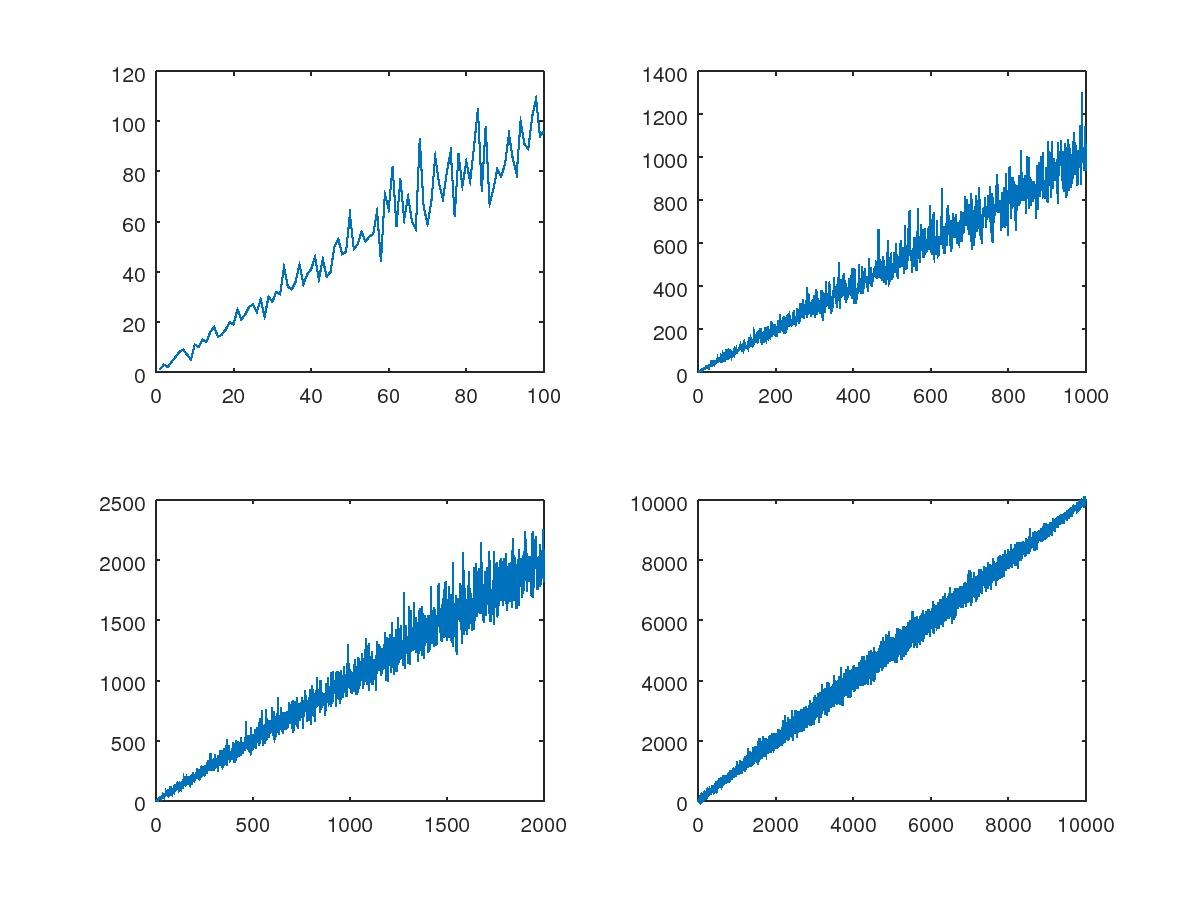
\includegraphics[width=\textwidth]{grafico_es4.jpeg}
	
	Possiamo notare che nelle prime e ultime componenti del vettore $w$ è presente un minor discostamento dalla bisettrice, mentre nelle posizioni centrali questo fenomeno è più evidente. Questo a mio avviso è causato da due fattori:
	\begin{itemize}
		\item Effetto bordo: le prime e le ultime posizioni del vettore di pagerank possono essere "spostate" dalla permutazione $w$ solo in un senso (nel caso delle prime ho che la posizione non può diminuire e analogamente per le ultime non può aumentare)
		\item Concentrazione dei valori di PageRank: osservando il grafico che plotta i valori di PageRank delle pagine in ordine (cioè plotta $val1$) si vede che la "derivata" di questa curva è maggiore all'inizio e alla fine, quindi le pagine nel "mezzo" del vettore $w$ hanno rank molto vicini e cambiare $\gamma$ fa variare molto di più le posizioni mediane che quelle estremali. 
			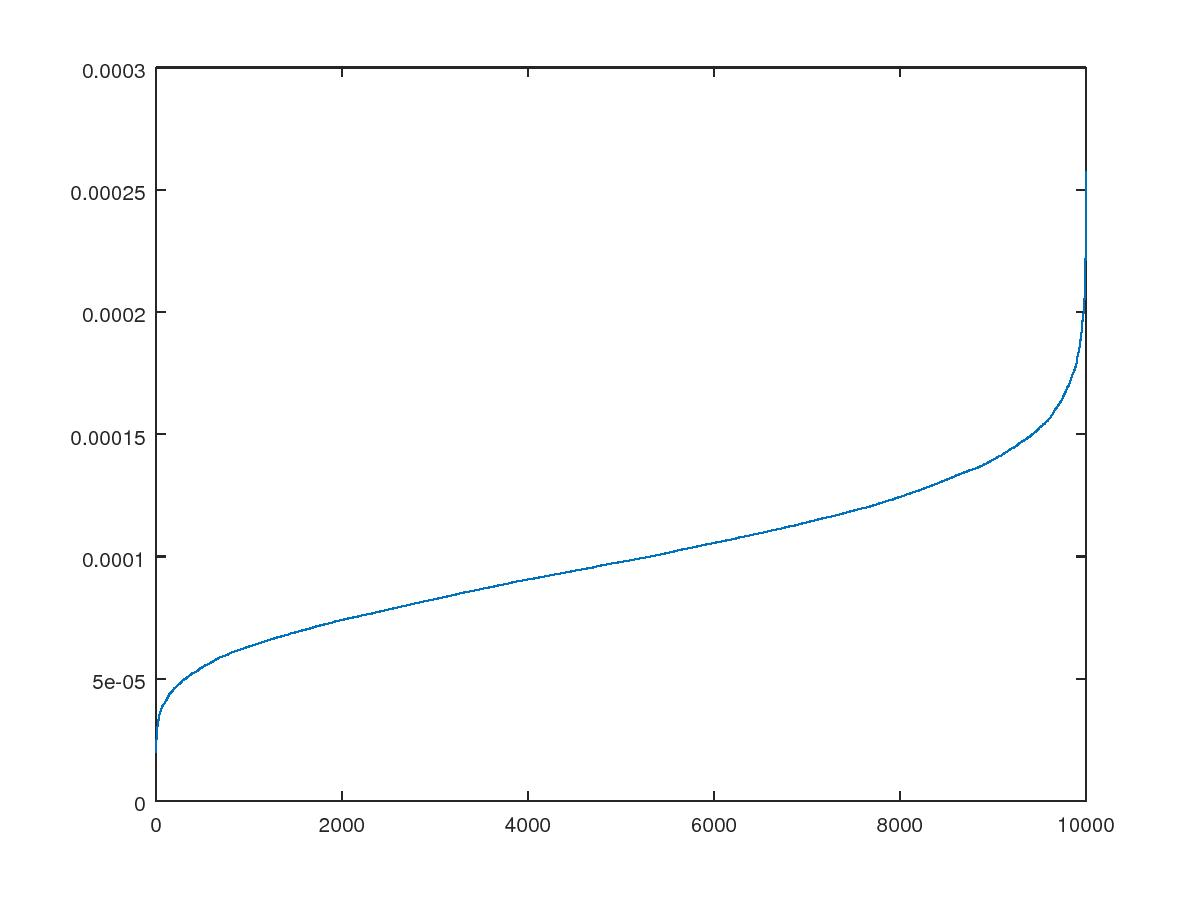
\includegraphics[width=\textwidth]{grafico_es4,1.jpeg}
	\end{itemize}
	\section{Sperimentazione variando $n$ e densità della matrice sparsa}
	Proviamo ora a variare la dimensione della matrice e la densità applicando sempre la stessa sperimentazione.
	\section{Lo script}
	Questo è lo script che realizza la sperimentazione:
	\lstinputlisting{s_es4o.m}
	Dove la funzione {\tt PageRank} è la solita funnzione usata nella precedente sperimentazione.
	\section{Risultati}
	Riportiamo i grafici di $w$ per i vari valori di $n$ e $n^2 \cdot d$ in sovraimpressione:
	
	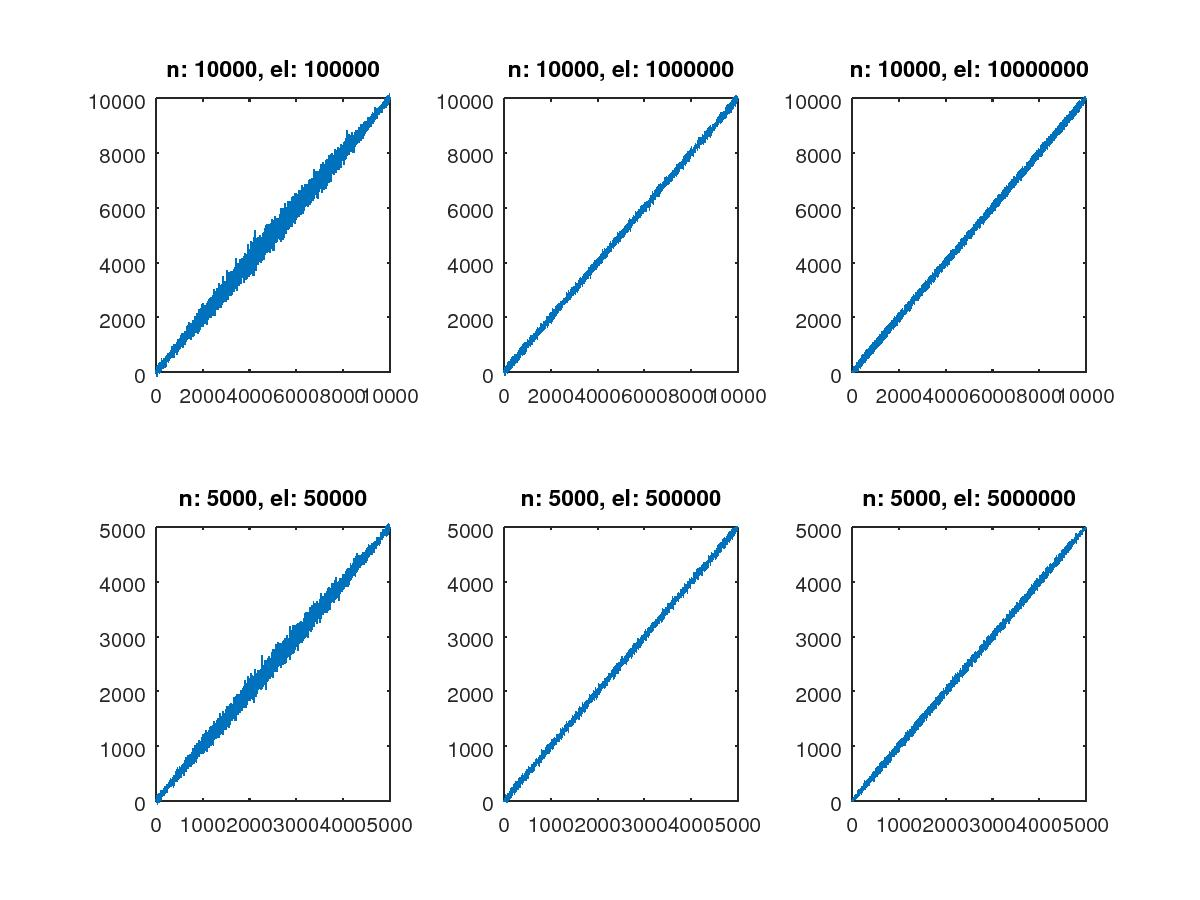
\includegraphics[width=\textwidth]{grafico_es4o.jpeg}
	Si può notare che aumentando il numero di elementi non nulli si ha un discostamento minore del grafico dalla bisettrice.
\end{document}